\section{Results and discussion}
\label{sec:results}

\subsection{Synthetic gray-scale data}
The proposed method solved precisely the specific challenge
created by the model. A severe distortion of the model is
artificially created adding complexity to the problem of
partial voluming in the outer contour of the sulcus.
\autoref{fig:sulcusmodel_result} provides visual assessment
for this result. With 16x16x16 control points and an 
approximate total of 29,000 nodes contained by the two prior 
surfaces, computation time for this model was around
14 minutes in an \textit{Intel\textsuperscript{\textregistered} 
Core\textsuperscript{\texttrademark} i5 CPU M 430 @ 2.27GHz} and
4GB RAM.

\begin{figure}
\begin{tabular}{ccccc}
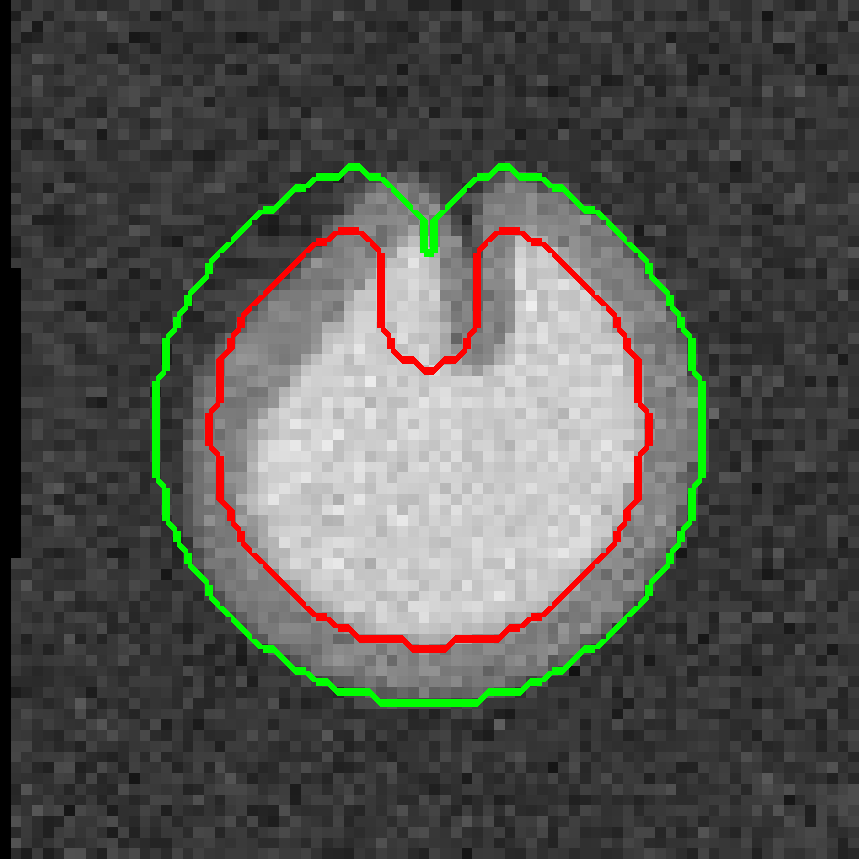
\includegraphics[width=0.19\textwidth]{model2result_b_1} &
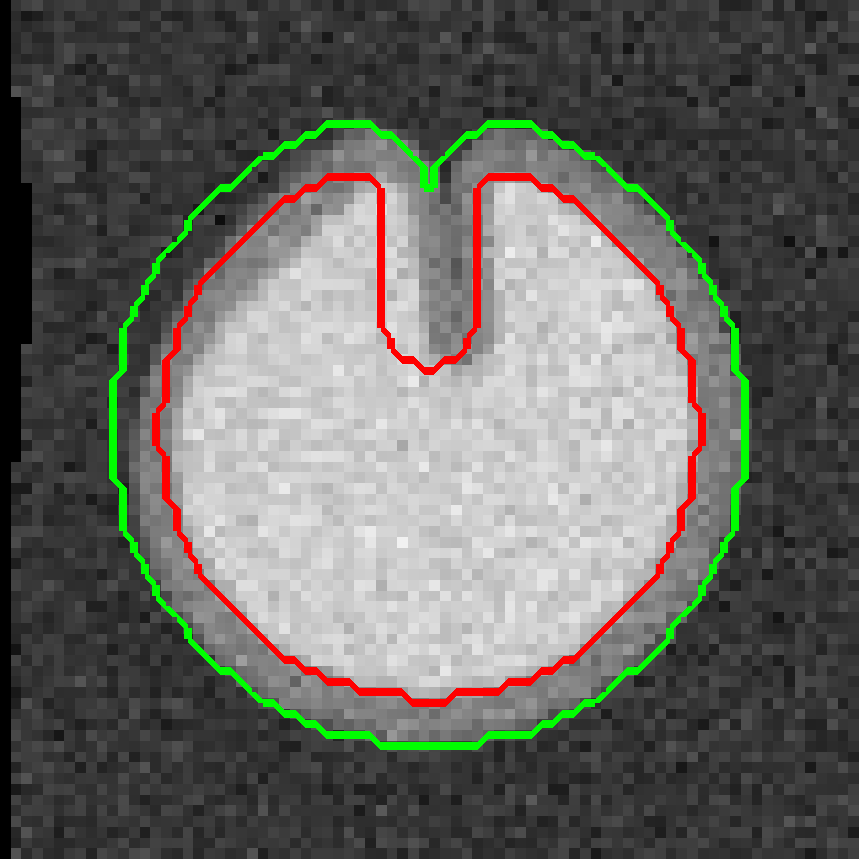
\includegraphics[width=0.19\textwidth]{model2result_b_2} &
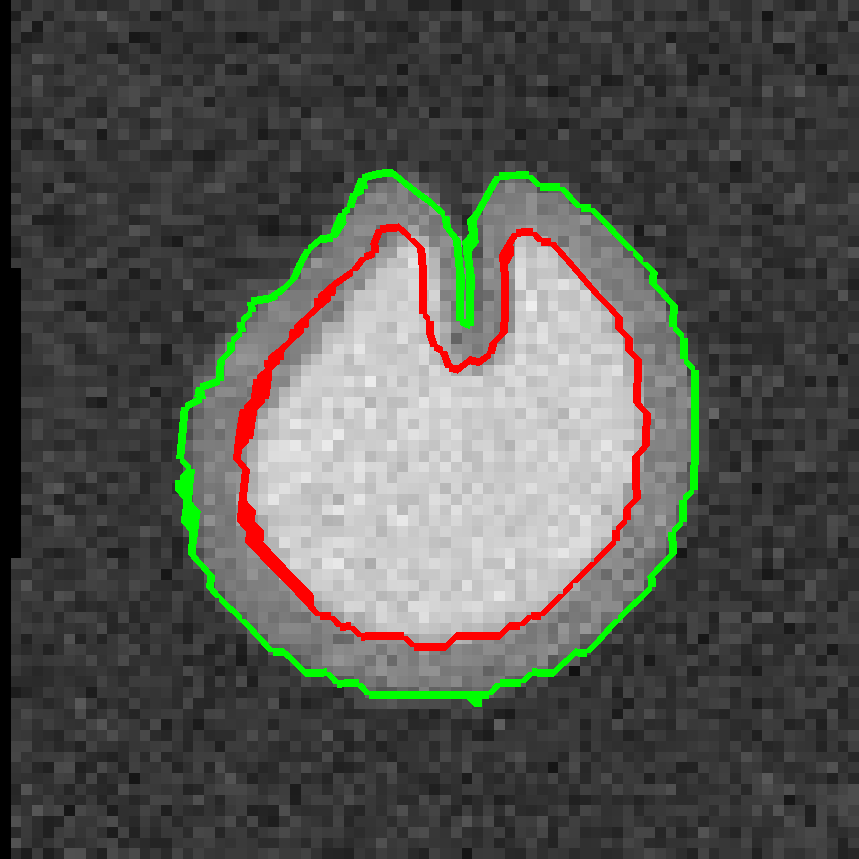
\includegraphics[width=0.19\textwidth]{model2result_a_1} &
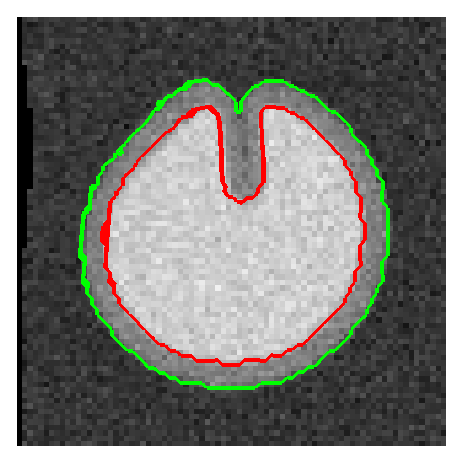
\includegraphics[width=0.19\textwidth]{model2result_a_2} &
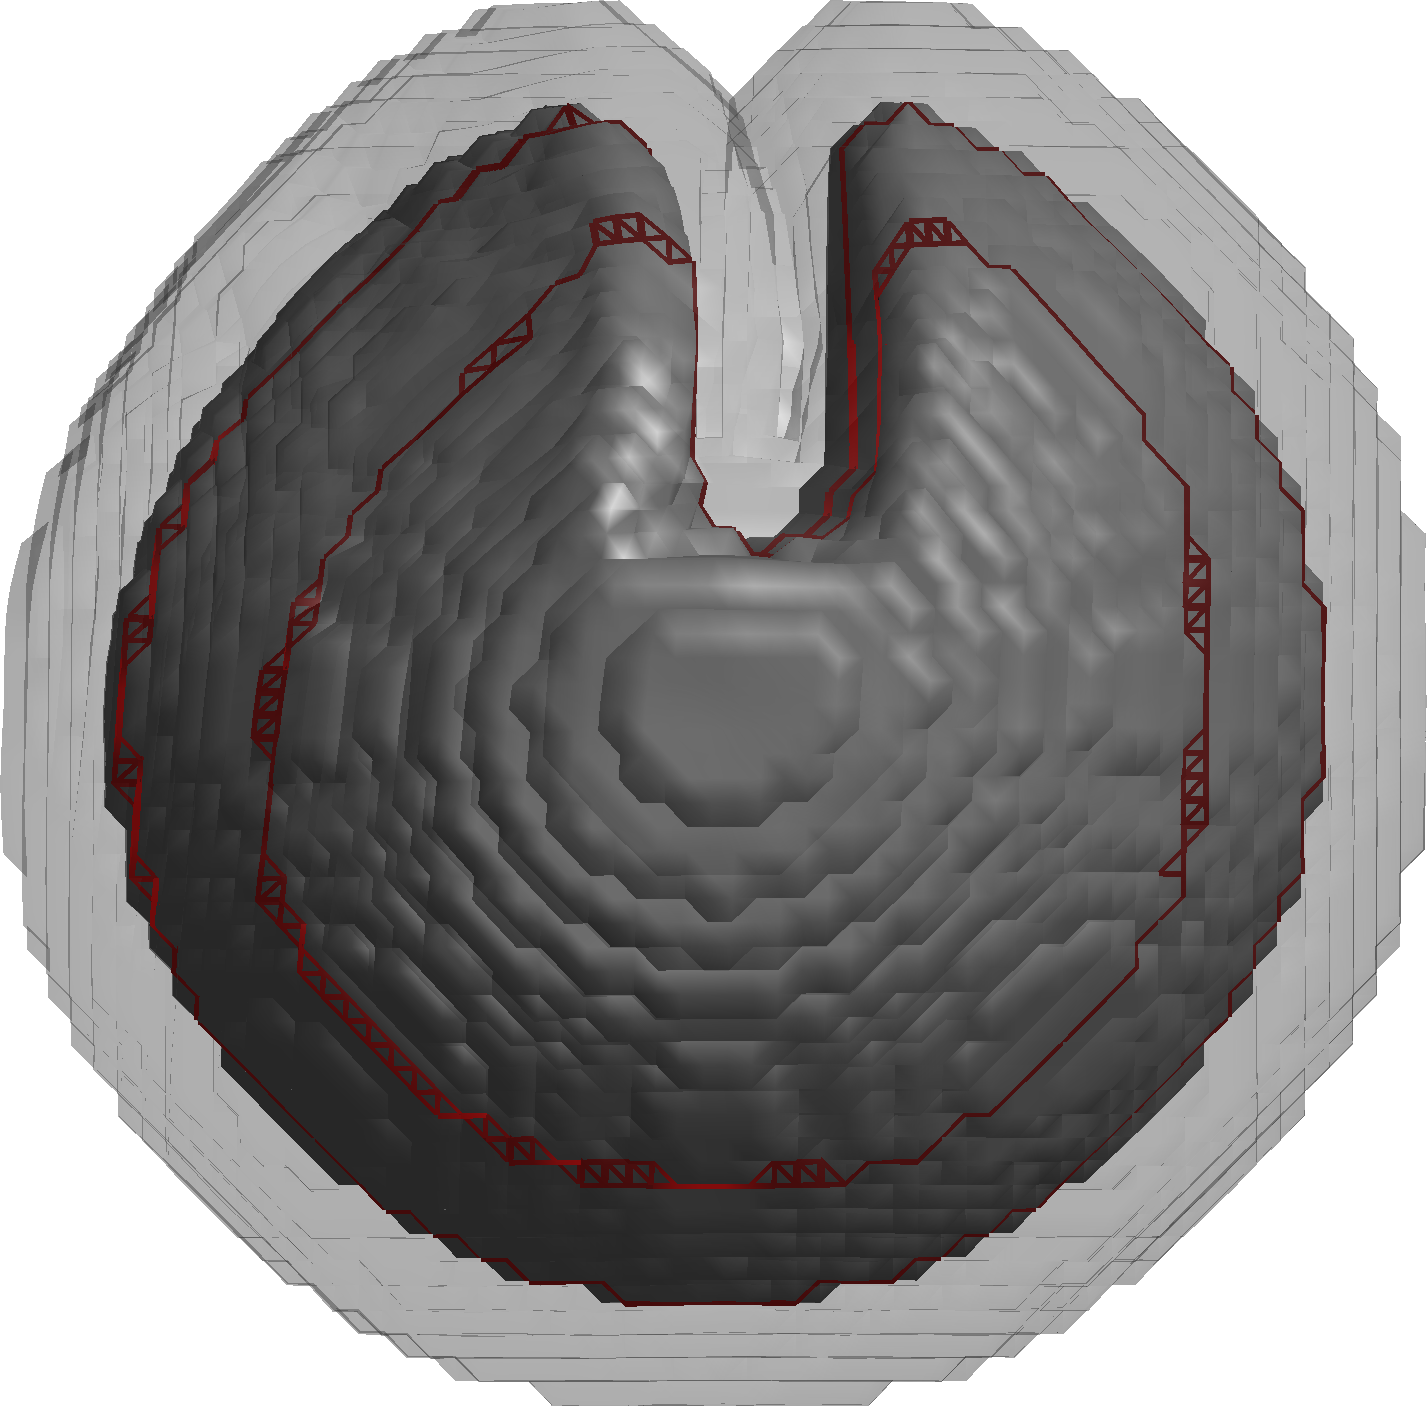
\includegraphics[width=0.19\textwidth]{model2surf} \\
\multicolumn{2}{c}{a)} & \multicolumn{2}{c}{b)} & c)
\end{tabular}
\caption{Result of the segmentation performance on the sulcus model.
a) Two slices and prior contours before segmentation-registration. b) The same slices and contours after distortion estimation. c) 3D rendering of the deformed priors, with the traces of the two selected slices highlighted.}
\label{fig:sulcusmodel_result}
\end{figure}


\subsection{Simulated diffusion data}
\label{sec:simulated_dwi}
%
The proposed method successfully reverted the synthetic distortion
field we applied to the data. Second row in \autoref{fig:fa} shows 
the fitted contours obtained by using the original surfaces of the model
as shape priors, with a constant translation of [5.0,10.0,-5.0] mm.
to illustrate briefly the extent of the capture range of the algorithm.
Computation time in this case was around 10 minutes in the previously
described platform, with 16x16x16 control points on
the dense deformation field and approximately 26,000 nodes in 
total for both prior surfaces. \\
%

%\begin{figure}
%\begin{tabular}{ccccc}
%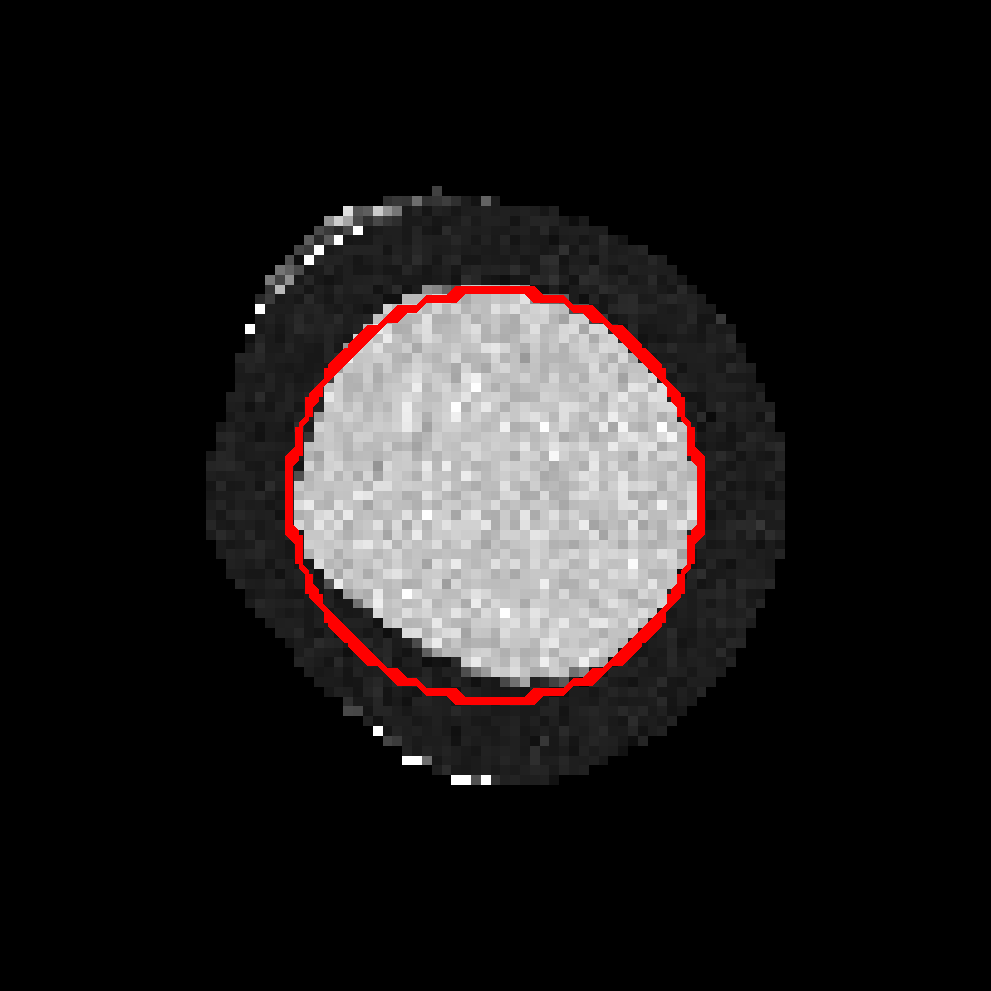
\includegraphics[width=0.19\textwidth]{model1result_b_1} &
%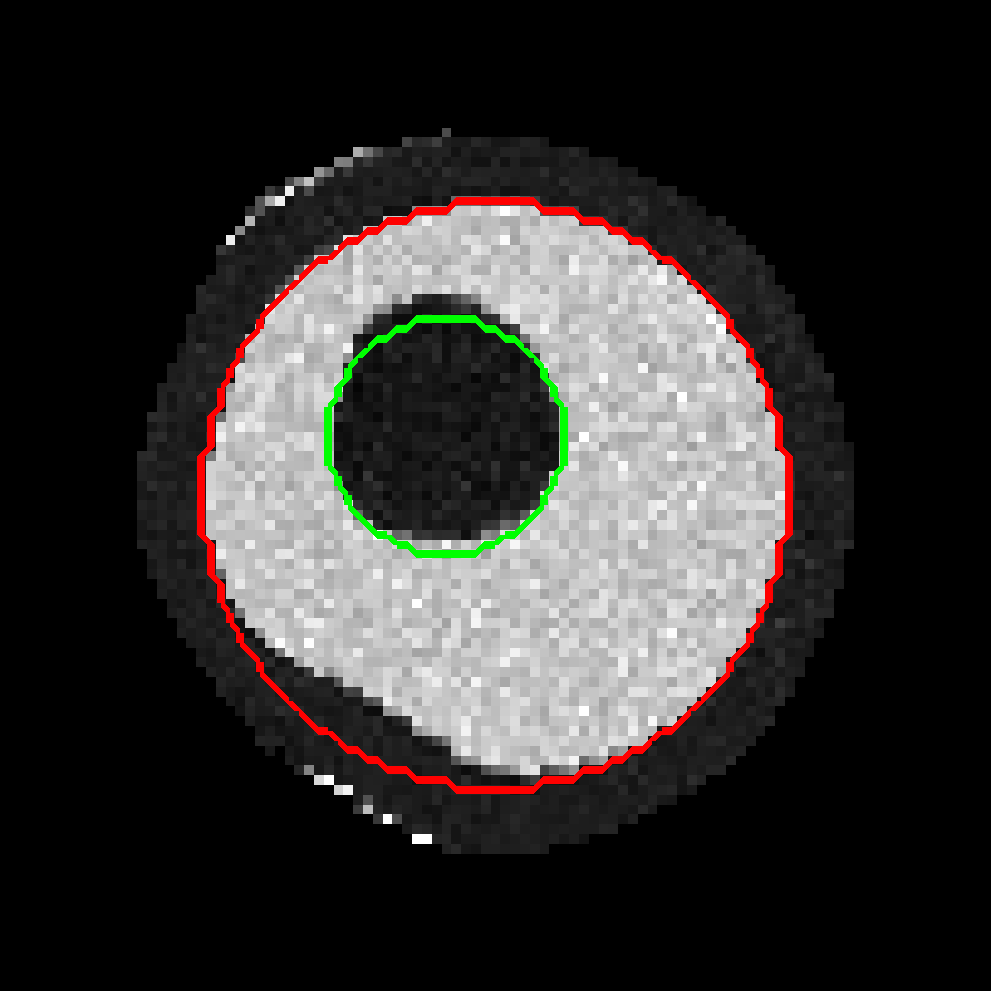
\includegraphics[width=0.19\textwidth]{model1result_b_2} &
%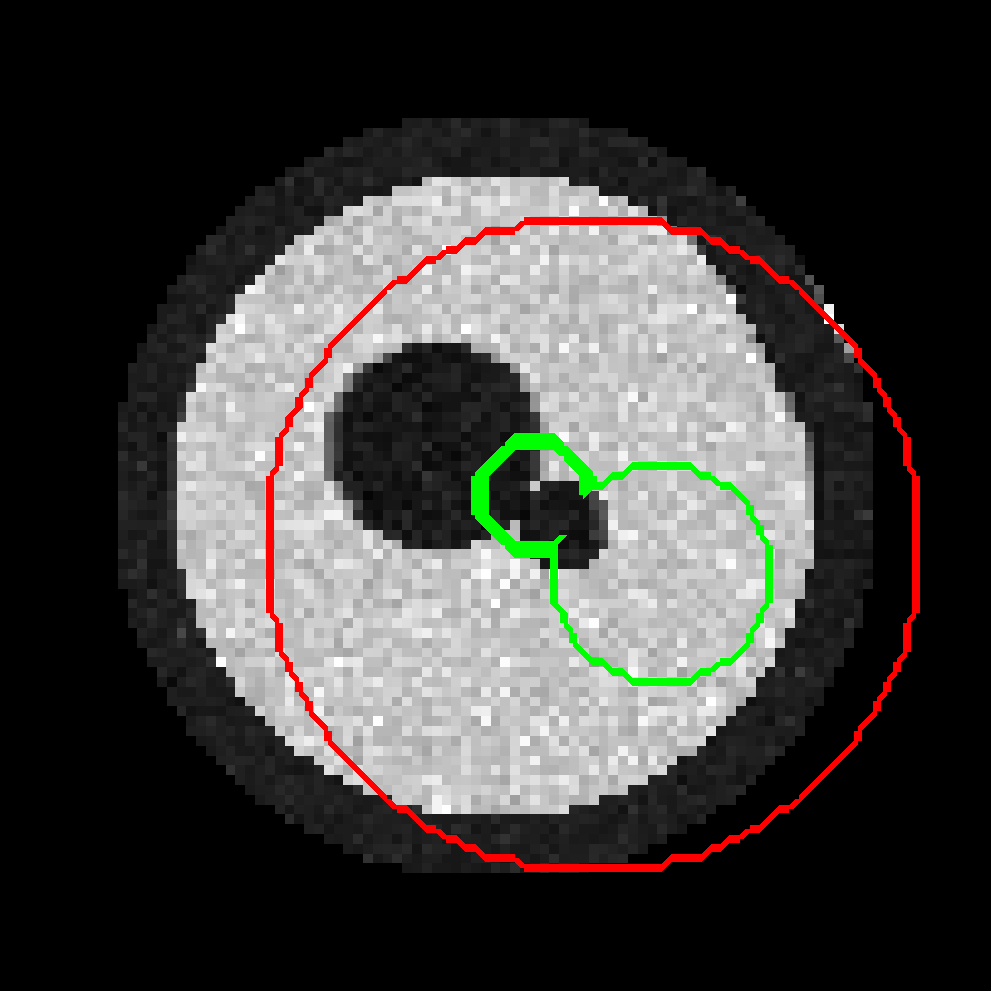
\includegraphics[width=0.19\textwidth]{model1result_b_3} &
%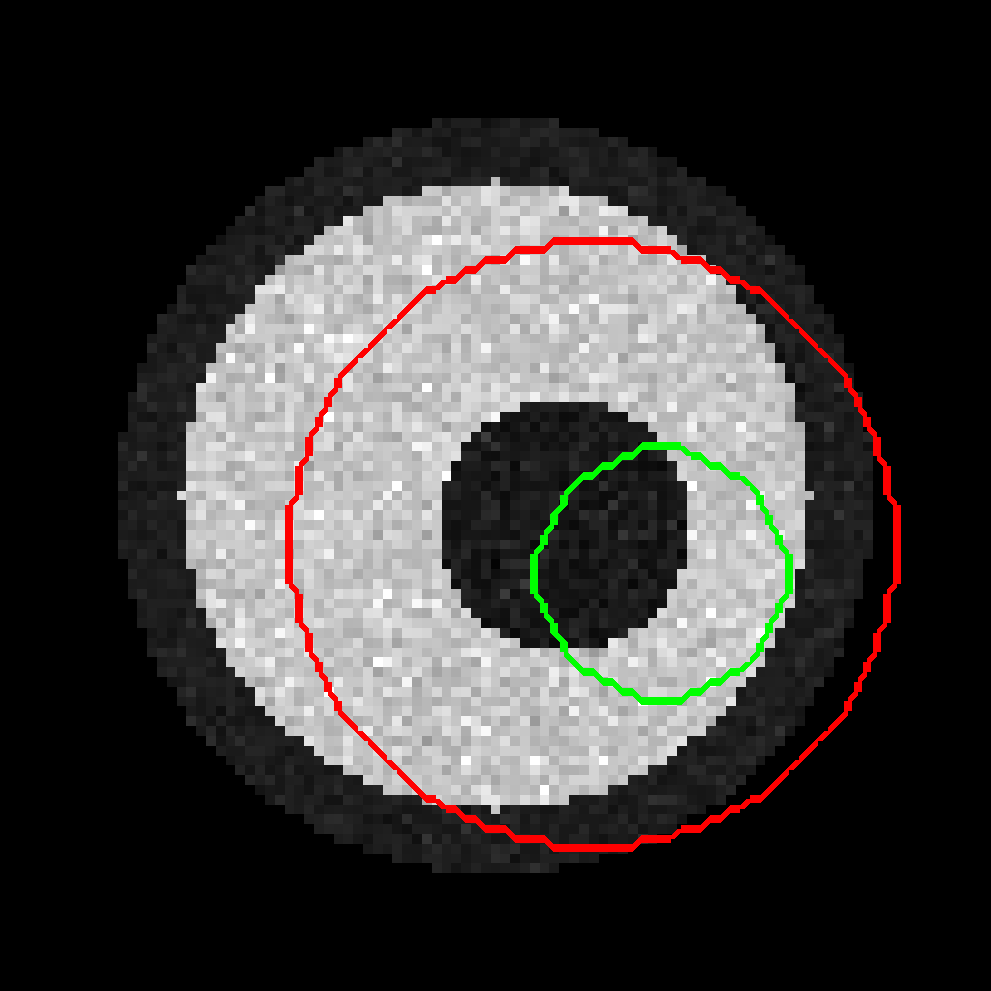
\includegraphics[width=0.19\textwidth]{model1result_b_4} &
%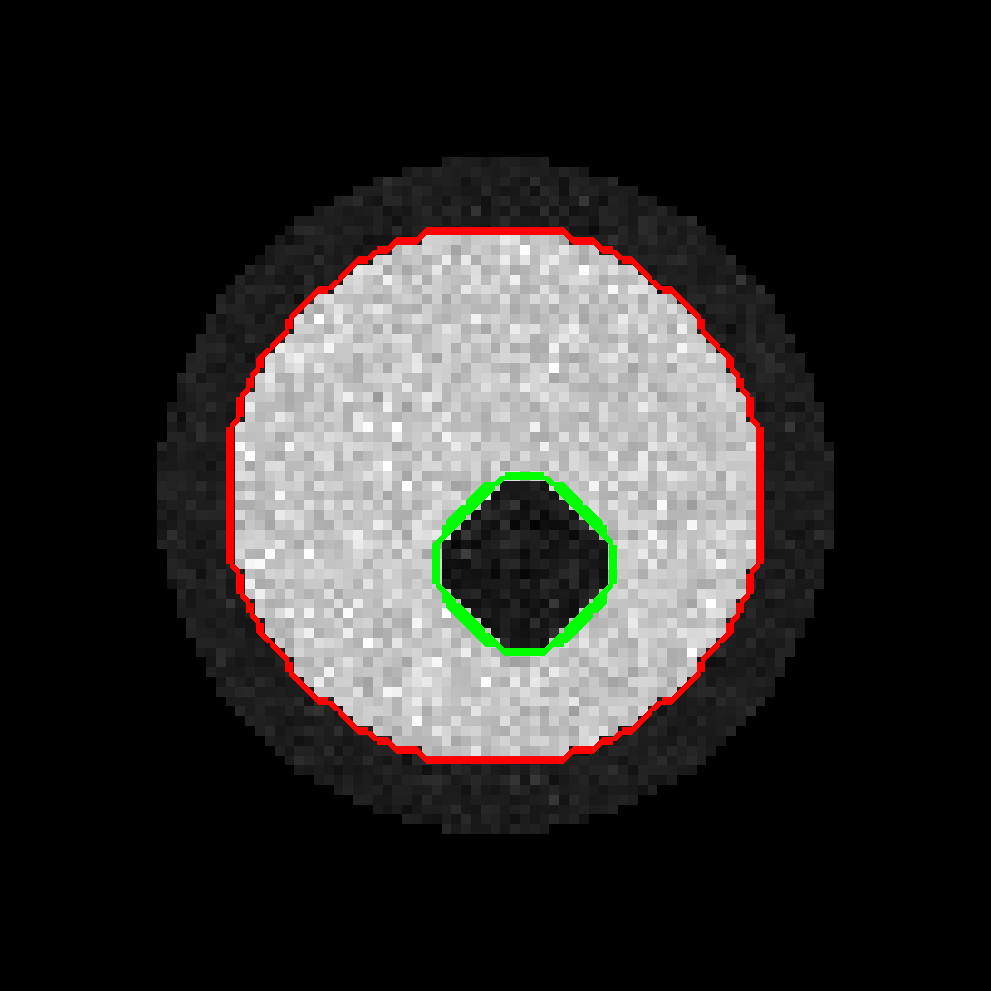
\includegraphics[width=0.19\textwidth]{model1result_b_5} \\
%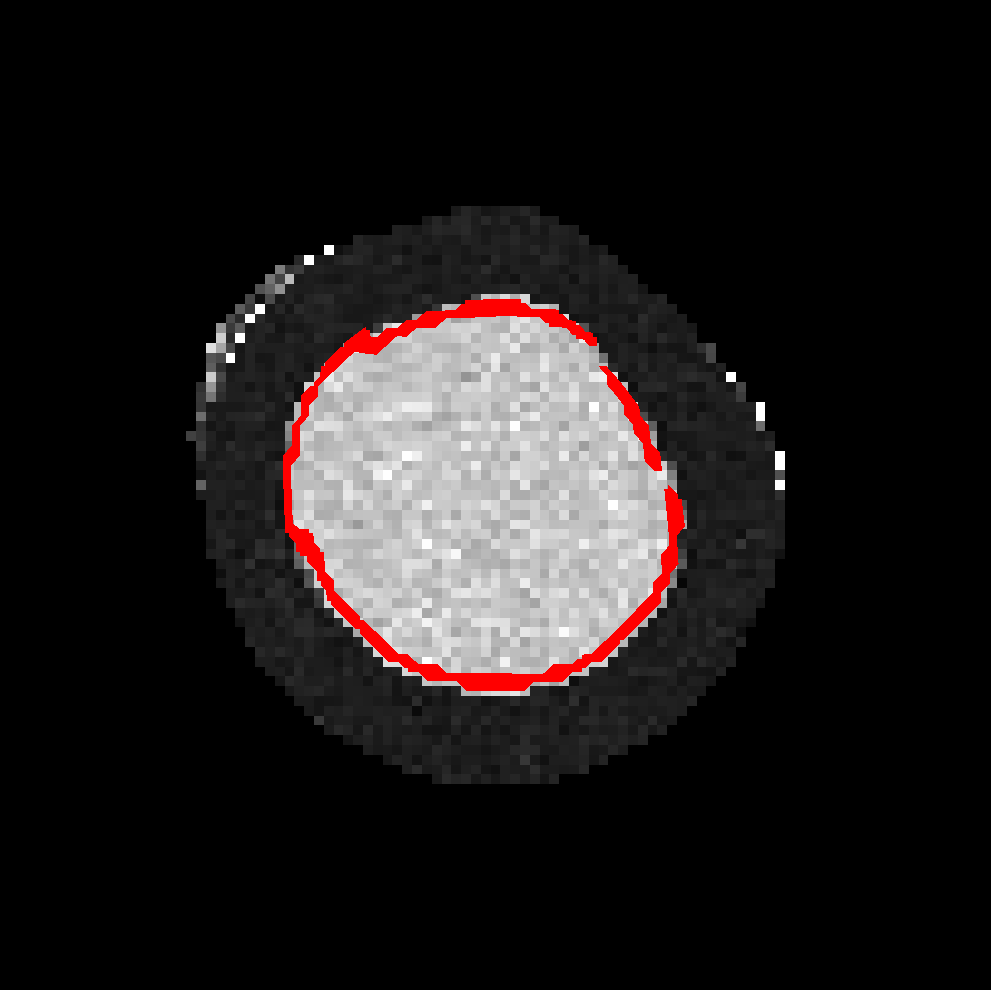
\includegraphics[width=0.19\textwidth]{IPMI2013-011} &
%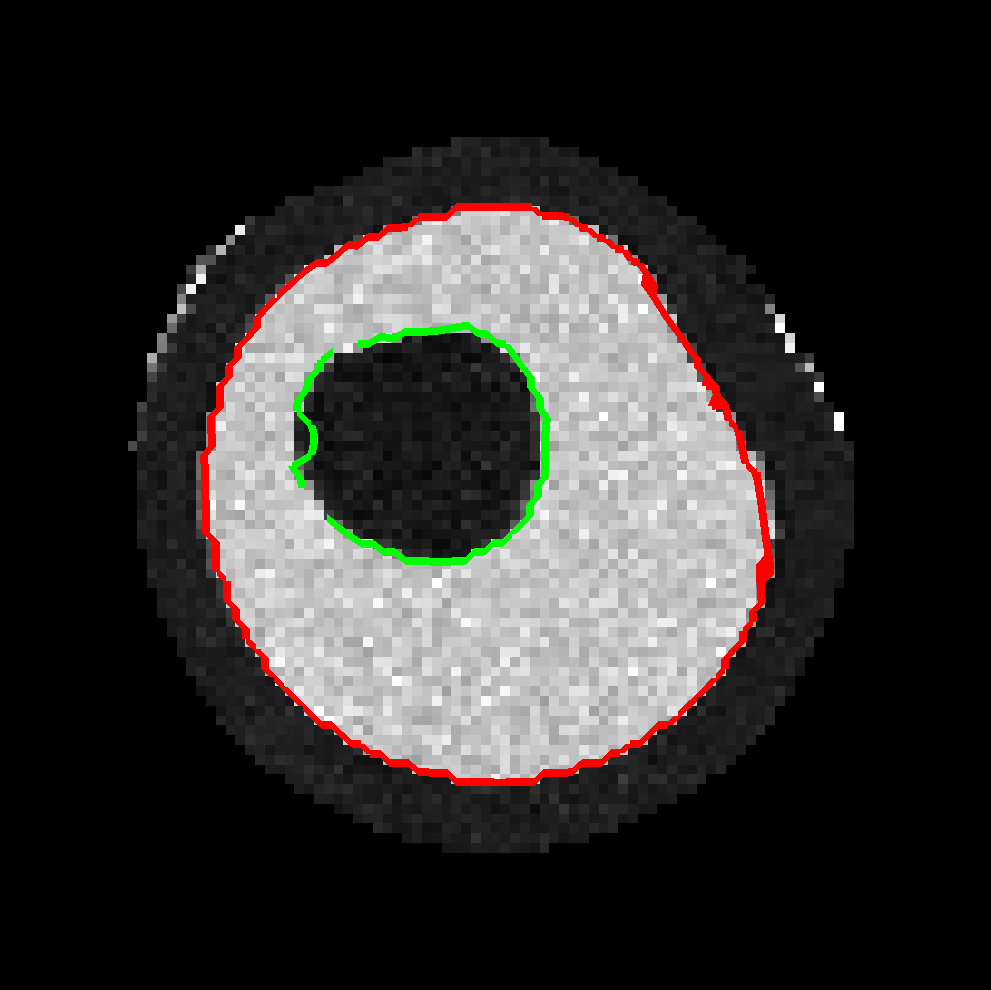
\includegraphics[width=0.19\textwidth]{IPMI2013-012} &
%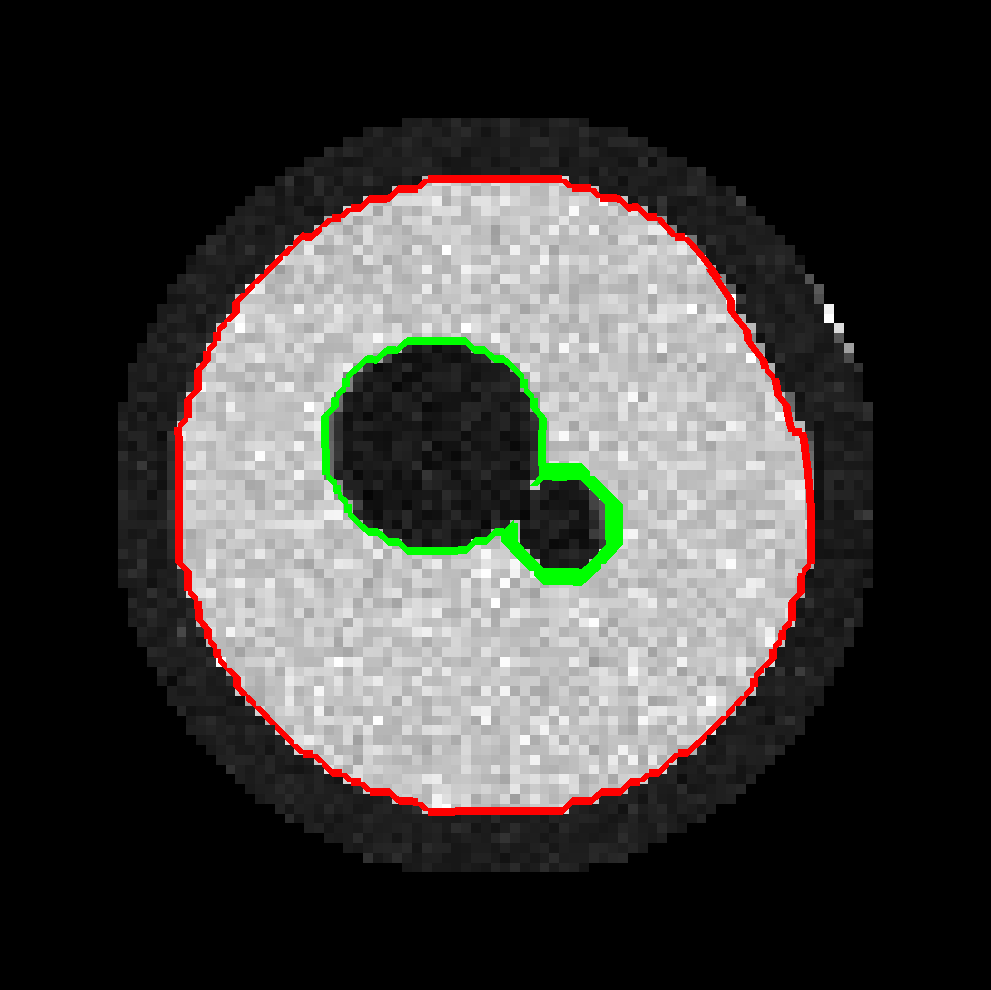
\includegraphics[width=0.19\textwidth]{IPMI2013-013} &
%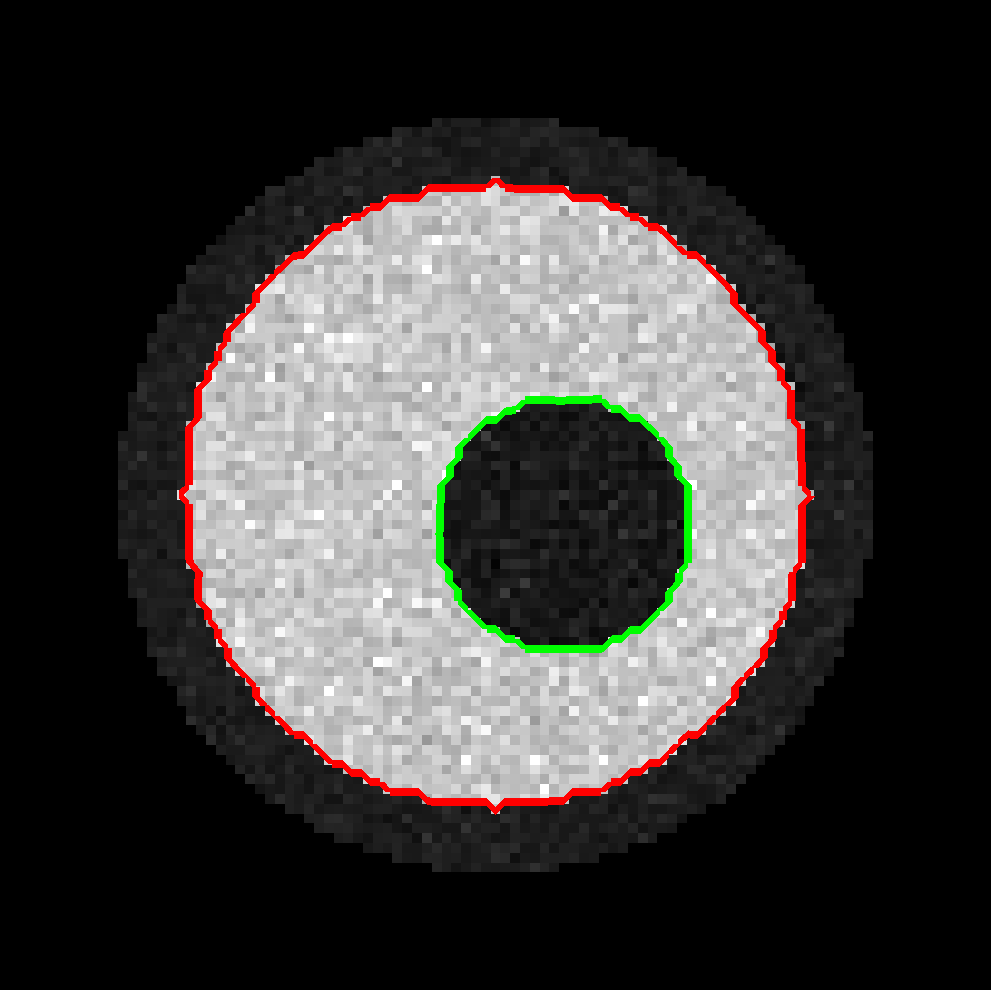
\includegraphics[width=0.19\textwidth]{IPMI2013-014} &
%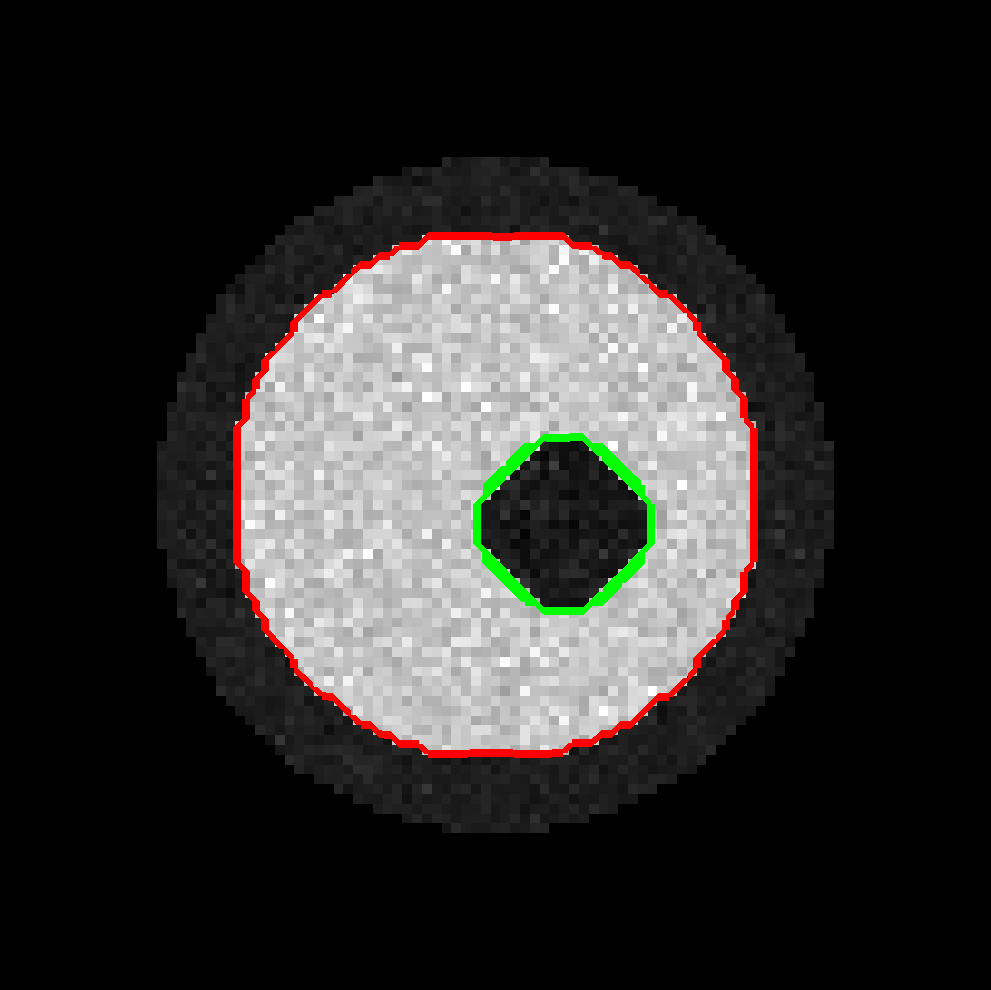
\includegraphics[width=0.19\textwidth]{IPMI2013-015} \\
%%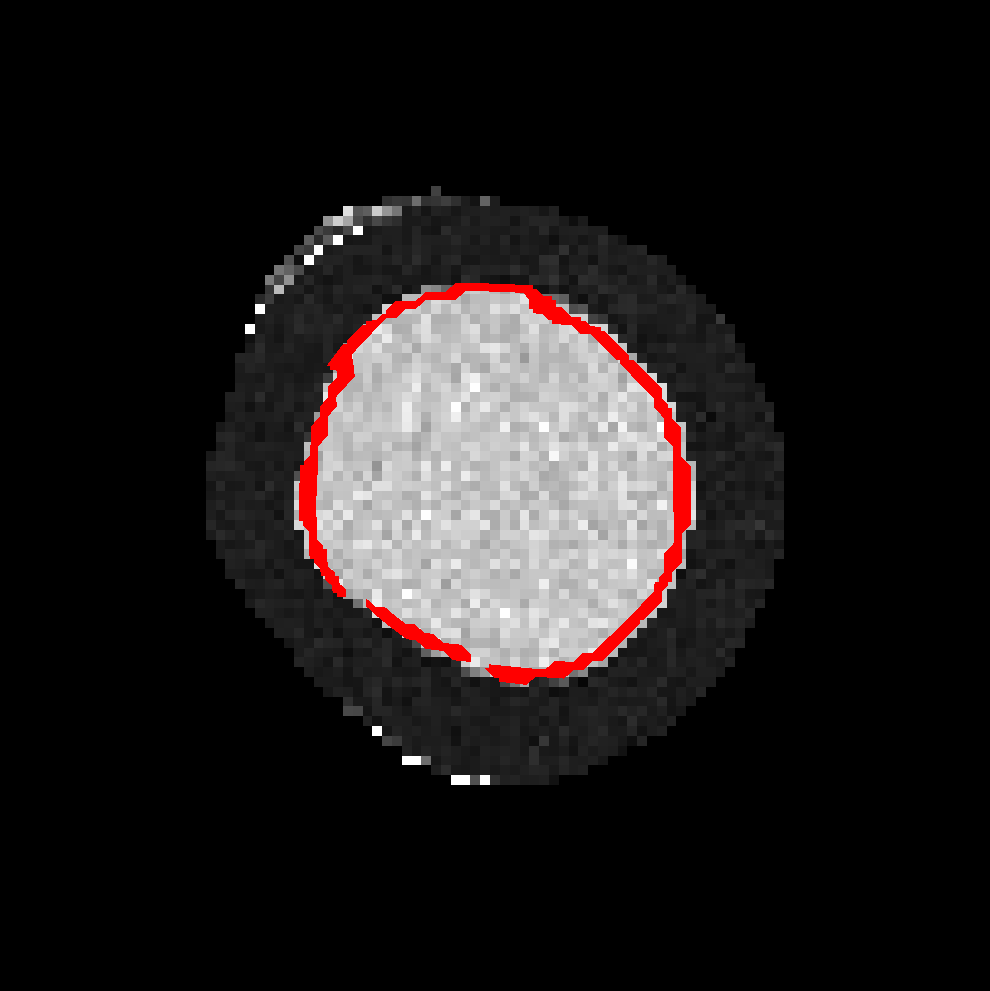
\includegraphics[width=0.19\textwidth]{model1result_a_1} &
%%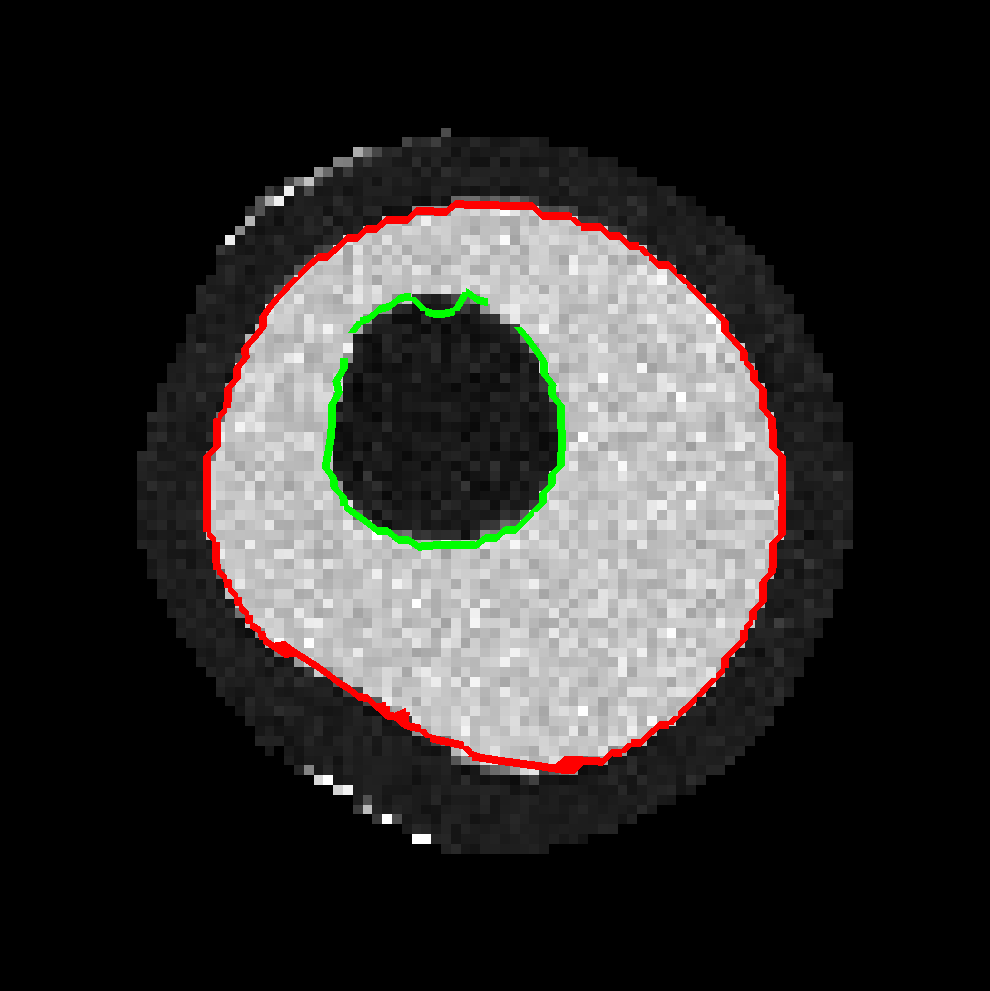
\includegraphics[width=0.19\textwidth]{model1result_a_2} &
%%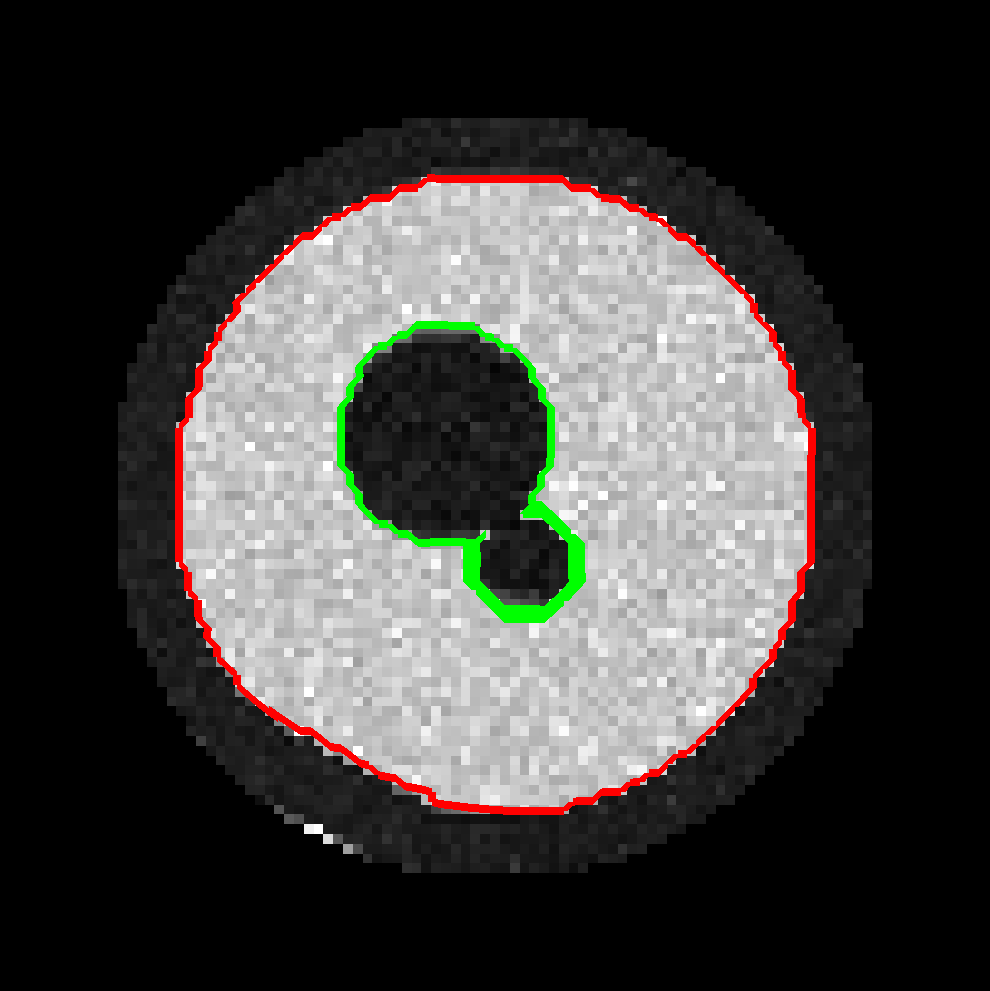
\includegraphics[width=0.19\textwidth]{model1result_a_3} &
%%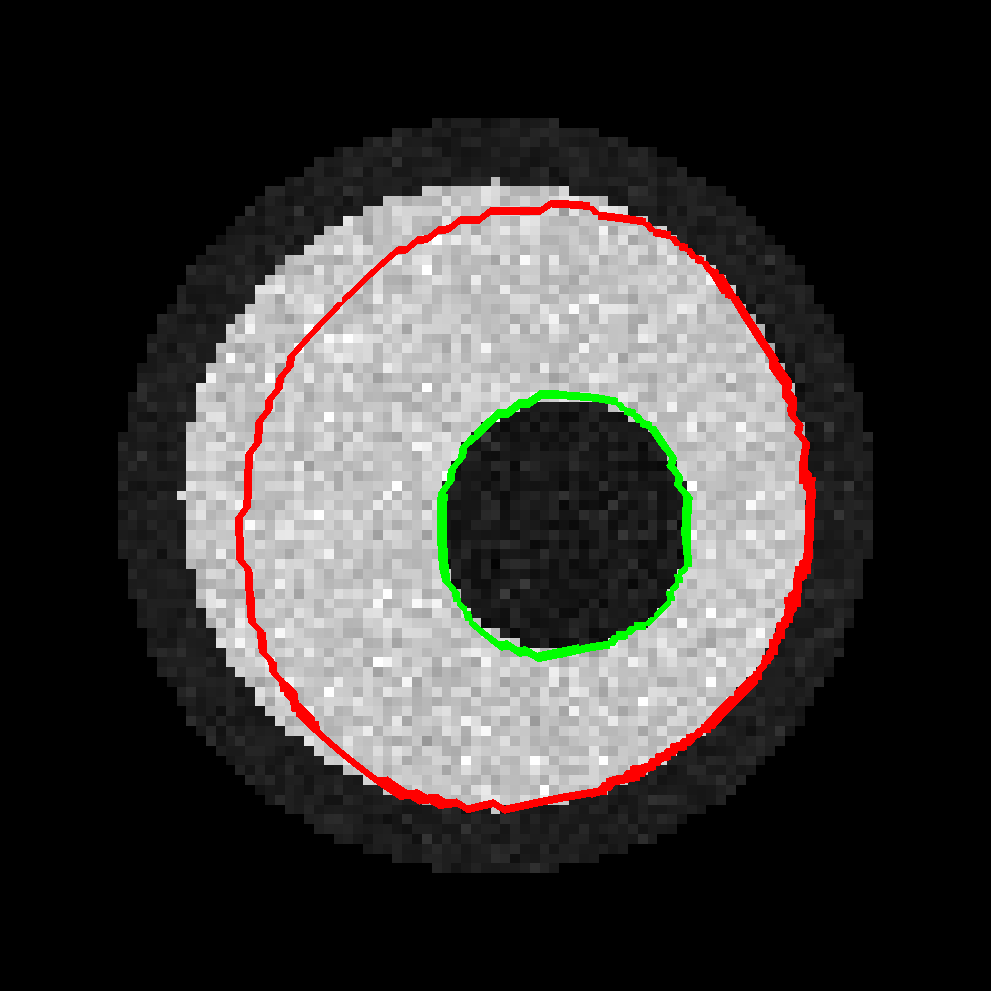
\includegraphics[width=0.19\textwidth]{model1result_a_4} &
%%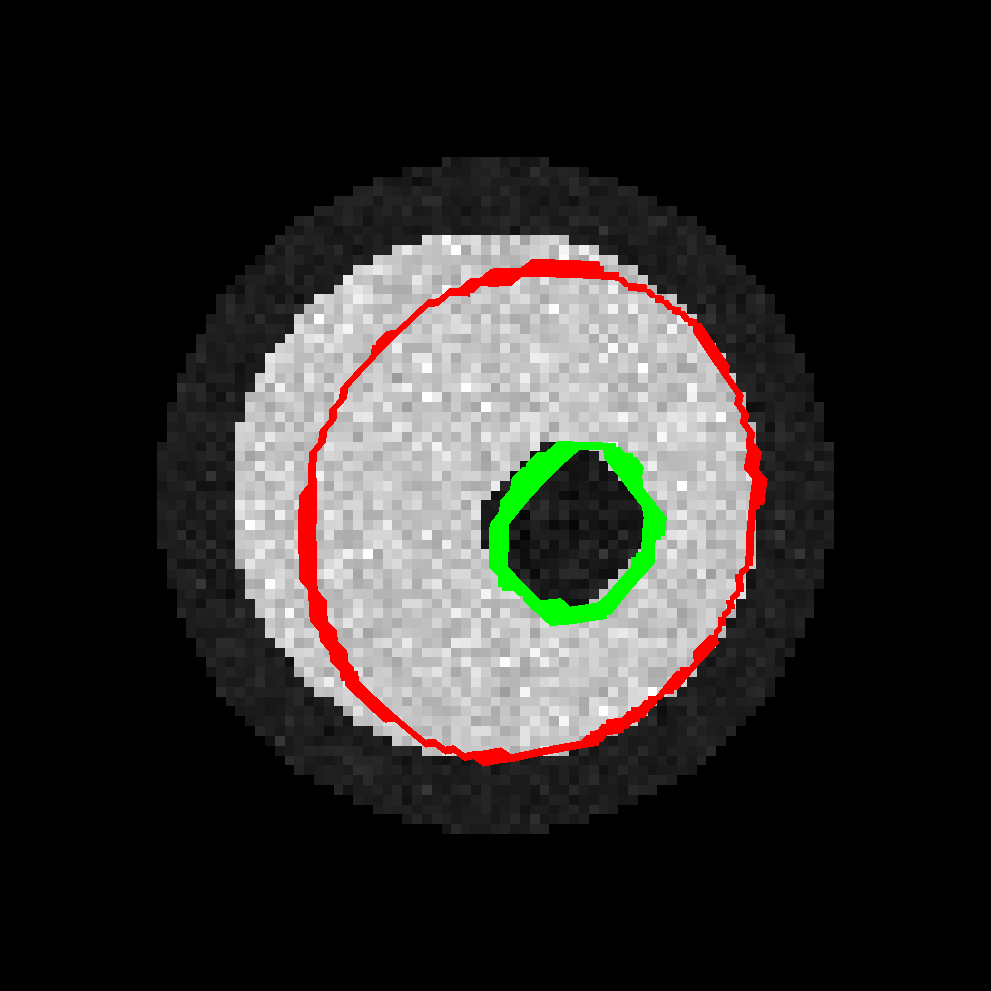
\includegraphics[width=0.19\textwidth]{model1result_a_5} \\
%\end{tabular}
%\caption{First row presents several slices along Z axis of the distorted \gls{fa} map and
%the undistorted \gls{wm}-\gls{gm} and \gls{wm}-\gls{csf} contours given as shape priors,
%subjected to the shift of [5.0,10.0,-5.0] mm. described in \autoref{sec:simulated_dwi}.
%Second row contains the same map, now with the contours after joint segmentation-registration.}
%\label{fig:fa}
%\end{figure}